\documentclass[conference]{IEEEtran}
\IEEEoverridecommandlockouts
% The preceding line is only needed to identify funding in the first footnote. If that is unneeded, please comment it out.
%Template version as of 6/27/2024

\usepackage{cite}
\usepackage{amsmath,amssymb,amsfonts}
\usepackage{algorithmic}
\usepackage{graphicx}
\usepackage{textcomp}
\usepackage{xcolor}
\usepackage{booktabs}
\def\BibTeX{{\rm B\kern-.05em{\sc i\kern-.025em b}\kern-.08em
    T\kern-.1667em\lower.7ex\hbox{E}\kern-.125emX}}

% Added manually:
\usepackage{tikz}
\usetikzlibrary{arrows.meta, positioning, fit}
\usepackage{hyperref}
    
\begin{document}

\title{Efficient Environment Exploration and 3D Reconstruction with Reinforcement Learning and Multiple View Geometry}

% 1\textsuperscript{st} % could be used for 1.
\author{\IEEEauthorblockN{Frank Zillmann}
\IEEEauthorblockA{\textit{Department of Computer Engineering} \\
\textit{Technical University of Munich (TUM)}\\
Munich, Germany \\
frank.zillmann@tum.de}
}

\maketitle

\begin{abstract}
Within this project the problem of autonomous 3D scene reconstruction is tackeled through a combination of reinforcement learning and classical multi-view geometry techniques.
A simulated Franka Panda robot equipped with a wrist-mounted RGB-D camera explores a tabletop scene containing randomly placed primitive objects.
Depth observations are incrementally fused into a Truncated Signed Distance Field (TSDF) using either Open3D or NVIDIA nvblox, and the resulting reconstruction is compared against a ground-truth mesh at every step---using Chamfer distance or a voxel-wise TSDF error---to compute the reward signal.
The robot policy predicting the robot motion can use multiple observations in a modular structure, among them the previous trajectory using a Transformer or renderings and uncertainty data of the current reconstruction using Convolutional Neural Networks, and is trained with Proximal Policy Optimization (PPO).
Experiments show that the policy useful strategies as moving up and sliding over the table, beating a simple scripted baseline. Challenges as little dependence on the configuration of objects on the table and missing long training runs due to memory leaks in the used libraries are discussed.
\end{abstract}

% \begin{IEEEkeywords}
% reinforcement learning, 3D reconstruction, active perception, TSDF, next-best-view planning
% \end{IEEEkeywords}

%======================================================================
\section{Introduction}

Reconstructing the 3D geometry of an environment from a sequence of depth or RGB-D images is a fundamental problem in robotics and computer vision.
Classical multi-view geometry pipelines such as Structure-from-Motion~\cite{schoenberger2016sfm} and volumetric fusion~\cite{curless1996volumetric} assume that images are collected by a human operator or a pre-programmed scanning trajectory.
In practice, the choice of viewpoints critically affects reconstruction quality: redundant views waste time while occluded regions remain unobserved.

% The \emph{next-best-view} (NBV) problem asks which camera pose should be selected next to maximally reduce reconstruction uncertainty.
% Traditional NBV methods rely on hand-crafted heuristics such as information gain or frontier-based exploration.
% Recently, learning-based approaches have emerged as a promising alternative, leveraging deep reinforcement learning (RL) to discover non-myopic viewpoint planning strategies directly from data~\cite{meli2025robotcellmodelingexploratory}.

Simultaneously, efficiently learning the 3D geometry of robot cells and workspaces to enable safe and effective operation is a critical capability for autonomous robots.
While other approaches try to tackle this problem through involving a human operator in the loop \cite{meli2025robotcellmodelingexploratory}, fully autonomous exploration and reconstruction is desirable for scalability and efficiency in frequently changing environments such manufacturing floors or laboratories.

In this work, a little framework was developed in which a simulated Franka Panda manipulator learns to move its wrist-mounted camera so as to maximize the reconstruction quality of a tabletop scene within a fixed episode horizon.
The main contributions are as follows:
\begin{itemize}
    \item A modular simulation environment built on robosuite~\cite{robosuite2020} including multiple reconstruction metrics and methods for reward shaping and computation of the ground-truth geometry.
    \item Integration of two volumetric reconstruction back-ends (Open3D~\cite{zhou2018open3d} and NVIDIA nvblox TODO citation) with a common interface
    \item A multi-input policy architecture that modulary fuses multiple observations spatial modalities (camera pose history, 2D images, 3D reconstruction uncertainty).
    \item A training pipeline using PPO that allows to flexibly choose reconstruction policy, reconstruction metric, obersavtions, and other hyperparameters using a environment wrapper with Gymnasium interface.
\end{itemize}

%======================================================================
\section{Related Work}

\textbf{Volumetric 3D Reconstruction.}\quad
Curless and Levoy~\cite{curless1996volumetric} introduced TSDF-based volumetric fusion, which remains the dominant paradigm for real-time depth integration.
Open3D~\cite{zhou2018open3d} provides a widely used open-source implementation based on voxel block grids, while NVIDIA's nvblox accelerates integration and querying on GPUs.
Neural implicit representations~\cite{Liao_2024_WACV, Guo_2024_UNIKD, Younes_2024_SparseCraft} offer an alternative but are currently too slow for online RL training loops.

\textbf{Next-Best-View Planning.}\quad
Classical Next-Best-View Planning methods greedily select the next viewpoint that maximizes an information-theoretic criterion.
This work follows a similar motivation but focuses on techniques for learning the next-best-view using Reinforcement Learning specifically with a robot arm but without specializing on a specific reconstruction method or training on a shape dataset.

\textbf{Reinforcement Learning and Robot Simulation.}\quad
PPO~\cite{schulman2017proximalpolicyoptimizationalgorithms} is a widely used on-policy algorithm that provides stable training with clipped surrogate objectives.
Stable-Baselines3~\cite{stable-baselines3} offers a reliable PPO implementation and is used in this work.
The robosuite simulator~\cite{robosuite2020} provides standardized manipulation environments with MuJoCo~\cite{todorov2012mujoco} physics and has been extended in this project with a custom reconstruction task.

%======================================================================
\section{Methods}
The system is decomposed into three components (Fig.~\ref{fig:architecture}):
\begin{itemize}
    \item \textbf{Robot Environment:} The simulated environment in which the robot operates, including the computation of the 3D reconstruction errors and rewards.
    \item \textbf{Reconstruction Policy:} The method used to reconstruct the 3D environment from the robot's observations.
    \item \textbf{Robot Policy:} The reinforcement learning policy and it's neural architecture that decides the robot's actions based on it several observations.
\end{itemize}

From a Reinforcement Learning perspective the combination of Robot Environment (\texttt{Reconstruct3D.py}) and Reconstruction Policy (\texttt{open3d\_TSDF\_generator.py} or \texttt{nvblox\_reconstruction\_policy.py}) can be seen as the total environment from a Reinforcement Learning perspective, while the Robot Policy is the agent that interacts with this environment. 
This approach is also taken in the code which uses the \texttt{reconstruct3D\_gym\_wrapper.py} to handle all necessary interactions between robot environment and reconstruction policy and the creation of the observations for the robot policy.

Alternative:

The system is decomposed into three components (Fig.~\ref{fig:architecture}): the \emph{Robot Environment}, which handles physics simulation and reward computation; the \emph{Reconstruction Policy}, which maintains the volumetric scene representation; and the \emph{Robot Policy}, the RL agent that selects actions.
A Gymnasium-compatible wrapper couples the first two into a single RL environment.

\begin{figure*}[t]
\centering
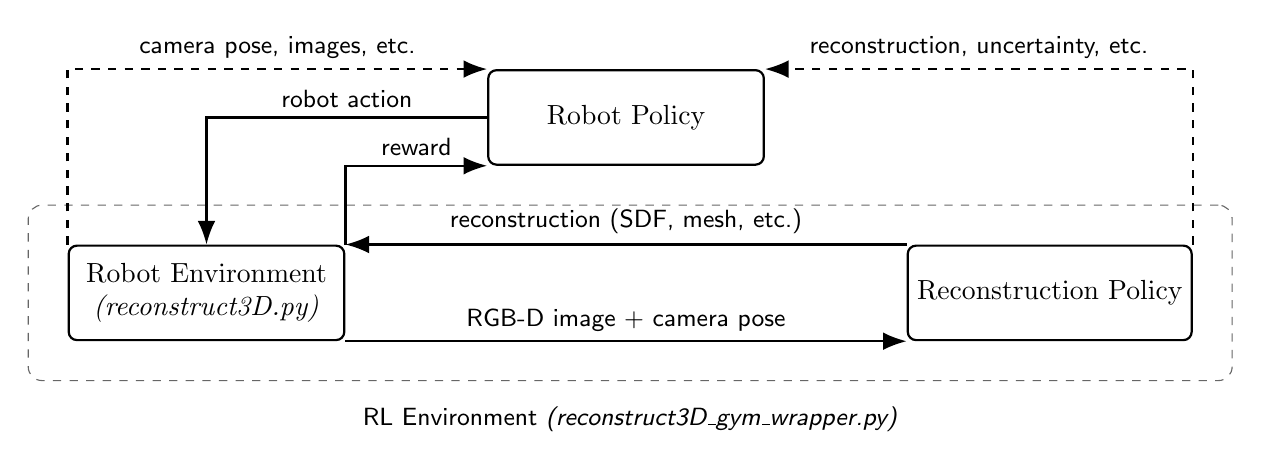
\begin{tikzpicture}[
  box/.style={draw, thick, rounded corners=3pt, minimum width=35mm, minimum height=12mm, align=center},
  arrow/.style={-{Latex[length=3mm]}, thick},
  dashedarrow/.style={-{Latex[length=3mm]}, thick, dashed},
  label/.style={font=\small\sffamily},
]

% --- Node placement (grid-like for zero clutter)
\node[box] (robot)                      {Robot Policy};
\node[box, below left=10mm and 18mm of robot]  (env)   {Robot Environment\\
\textit{(reconstruct3D.py)}};
\node[box, below right=10mm and 18mm of robot] (recon) {Reconstruction Policy};

% --- RL observation region
% \node[
%   draw=blue!60, dashed, rounded corners=5pt,
%   fit=(env)(recon),
%   inner sep=5mm,
% ] (group) {};

\node[
  draw=black!60, dashed, rounded corners=5pt,
  fit=(env)(recon),
  inner sep=5mm,
] (group) {};

\node[
  below=2mm of group,
  label,
  align=center,
  text width=80mm
] {
  RL Environment \textit{(reconstruct3D\_gym\_wrapper.py)}
};

% --- Arrows

\draw[arrow] (robot.west) -| node[label, near start, above]
  {robot action} (env.north);

\draw[arrow] (env.north east) |- node[label, near end, above]
  {reward} (robot.south west);

\draw[arrow] (env.south east) |- node[label, near end, above]
  {RGB-D image + camera pose} (recon.south west);

\draw[arrow] (recon.north west) |- node[label, near end, above]
  {reconstruction (SDF, mesh, etc.)} (env.north east);

% --- Arrows for observations

\draw[dashedarrow] (env.north west) |- node[label, near end, above]
  {camera pose, images, etc.} (robot.north west);

\draw[dashedarrow] (recon.north east) |-
  node[label, near end, above] {reconstruction, uncertainty, etc.} (robot.north east);

\end{tikzpicture}
\caption{System architecture. Solid arrows show the simulation loop; dashed arrows show observation flow to the RL agent. The wrapper encapsulates the environment and reconstruction module behind a standard Gymnasium interface.}
\label{fig:architecture2}
\end{figure*}

%----------------------------------------------------------------------
\subsection{Robot Environment}
%----------------------------------------------------------------------

The environment is built on robosuite~\cite{robosuite2020} with MuJoCo physics.
A Franka Panda 7-DoF manipulator is placed in front of a table ($1.0 \times 1.0$\,m) on which 2--4 primitive objects (boxes and cylinders of randomized sizes in $[0.05, 0.2]$\,m) are placed at random positions and orientations at each episode reset.
The robot carries an RGB-D camera on its end-effector (tool center point, TCP).

\textbf{Action Space.}\quad
The robot is controlled via an Operational Space Controller (OSC\_POSE) that accepts 6-DoF delta commands $\mathbf{a} = [\Delta x, \Delta y, \Delta z, \Delta r_x, \Delta r_y, \Delta r_z] \in [-1, 1]^6$ in the robot base frame.
These are scaled to position deltas of $\pm 0.05$\,m and orientation deltas of $\pm 0.25$\,rad per control step.
The control frequency is 4\,Hz relative to the MuJoCo simulation, and the default episode horizon is 32 steps (8\,s of simulated time).

\textbf{Ground Truth.}\quad
At each episode reset, the ground-truth mesh of the static scene (table plus objects) is extracted from MuJoCo's collision geometry, and its axis-aligned bounding box (with 5\% padding) defines the reconstruction volume.
For the voxel-wise TSDF metric, the ground-truth SDF is additionally computed on a $32^3$ grid via \texttt{mesh2sdf}~\cite{marian42_mesh_to_sdf}.

%----------------------------------------------------------------------
\subsection{Reconstruction Policy}
%----------------------------------------------------------------------

At every simulation step, the wrapper extracts the wrist camera's depth image, intrinsic matrix, and extrinsic pose, and passes them to the reconstruction back-end.
Two back-ends are supported:

\textbf{Open3D TSDF}~\cite{zhou2018open3d}: Uses the tensor-based \texttt{VoxelBlockGrid} API for depth-only integration with configurable voxel size, truncation distance, and maximum depth.
Mesh extraction is performed via marching cubes.
This back-end runs on CPU or GPU and requires no NVIDIA-specific drivers.

\textbf{NVIDIA nvblox}: Provides GPU-accelerated TSDF integration and direct voxel querying.
Beyond mesh extraction, nvblox supports querying the TSDF and observation weights on a dense grid, which enables the voxel-wise TSDF error metric and weight-grid observations.

Both back-ends share a common interface (\texttt{BaseReconstructionPolicy}) with \texttt{add\_obs}, \texttt{reconstruct}, and \texttt{reset} methods, making the choice transparent to the rest of the pipeline.
Default parameters are a voxel size of 0.01\,m, a truncation distance of 0.04\,m, and a maximum integration depth of 1.0\,m.

%----------------------------------------------------------------------
\subsection{Reconstruction Metrics and Reward Function}
\label{sec:reward}
%----------------------------------------------------------------------

Two error metrics quantify the deviation of the current reconstruction from the ground truth:

\textbf{Chamfer Distance (CD).}\quad
10\,000 points are sampled uniformly from both the reconstructed and ground-truth mesh surfaces via area-weighted barycentric sampling.
KD-trees are used for nearest-neighbor queries, and the metric is the symmetric mean $L_1$ distance:
\begin{equation}
    \mathrm{CD} = \frac{1}{2}\!\left(\frac{1}{N}\!\sum_{i=1}^{N}\!\min_{\mathbf{q}}\|\mathbf{p}_i - \mathbf{q}\|_1 + \frac{1}{N}\!\sum_{j=1}^{N}\!\min_{\mathbf{p}}\|\mathbf{q}_j - \mathbf{p}\|_1\right)
\end{equation}
where $\{\mathbf{p}_i\}$ and $\{\mathbf{q}_j\}$ are the sampled point sets.

\textbf{Voxel-wise TSDF Error.}\quad
The reconstructed TSDF is queried on the same $32^3$ grid as the ground truth.
The error has two components: (i)~the mean $L_1$ distance between observed TSDF values and the ground-truth SDF, and (ii)~a missing-voxel penalty equal to the fraction of near-surface voxels (ground-truth $|\text{SDF}| < 0.5 \cdot d_\text{trunc}$) that remain unobserved.
Voxels below the table surface are excluded to avoid penalizing physically inaccessible regions.

\textbf{Reward Shaping.}\quad
Two modes translate the error $e_t$ into a per-step reward:
\begin{itemize}
    \item \emph{Exponential}: $r_t = s \cdot \exp(-e_t / c)$, where $s$ is a scale and $c$ the characteristic error.
    \item \emph{Delta}: $r_t = s \cdot (e_{t-1} - e_t) / c$, which directly rewards error reduction.
\end{itemize}
An optional action penalty $\lambda \cdot \overline{|\mathbf{a}_t|}$ discourages unnecessarily large motions.
The delta mode was found to provide a clearer learning signal and is used in the final configuration.

%----------------------------------------------------------------------
\subsection{Robot Policy Architecture}
\label{sec:policy}
%----------------------------------------------------------------------

The policy uses a \emph{MultiInputPolicy} (Stable-Baselines3~\cite{stable-baselines3}) with a modular feature extraction front-end (\texttt{CombinedExtractor}) that fuses information from multiple observation modalities.
Each sub-extractor processes a different observation key and produces a fixed-dimensional feature vector; the concatenated result is projected through a linear layer to a 256-dimensional combined representation, which is then fed into the shared policy and value network heads (two hidden layers of 256 units each).

The following sub-extractors are used:

\textbf{Camera Pose History (Transformer).}\quad
The sequence of 7-DoF camera poses (position + quaternion) collected during the episode is processed by a small Transformer encoder (1 layer, 4 heads, $d_\text{model}=64$).
Positional embeddings are added, zero-padded future steps are masked, and the output is mean-pooled over valid time steps.
This allows the policy to reason about where the camera has already been, avoiding redundant revisits.

\textbf{Image Features (CNN).}\quad
A birdview RGB image from a fixed overhead camera and a grayscale rendering of the current reconstruction mesh are concatenated channel-wise and processed by a three-layer CNN (stride-2 convolutions with batch normalization, followed by adaptive average pooling), yielding a 128-dimensional feature vector.
Images are resized to $64 \times 64$ in the forward pass.

\textbf{Weight Grid (3D-CNN).}\quad
When using nvblox, the per-voxel observation weight grid ($32^3$, indicating how often each voxel has been observed) is processed by a three-layer 3D-CNN.
Weights are log-scaled ($\ln(1+w)$) before passing through the network.
This provides the policy with explicit spatial information about which parts of the scene lack observations.

%----------------------------------------------------------------------
\subsection{Training}
%----------------------------------------------------------------------

Training uses PPO with the hyperparameters listed in Table~\ref{tab:hyperparams}.
A single environment instance is used for data collection, and a separate evaluation environment with deterministic seeding logs images, meshes, and rewards every 50\,000 steps.

\begin{table}[t]
\centering
\caption{PPO Hyperparameters}
\label{tab:hyperparams}
\begin{tabular}{@{}ll@{}}
\toprule
Parameter & Value \\
\midrule
Horizon (steps/episode) & 32 \\
Control frequency & 4\,Hz \\
Parallel environments & 4 \\
Rollout length ($n_\text{steps}$) & 512 per env \\
Minibatch size & 128 \\
Epochs per update & 5 \\
Learning rate & $3 \times 10^{-4}$ \\
Discount factor $\gamma$ & 0.98 \\
GAE $\lambda$ & 0.95 \\
Clip range & 0.2 \\
Entropy coefficient & 0.01 \\
Total timesteps & $2 \times 10^6$ \\
Reward mode & delta \\
Action penalty $\lambda$ & 0.1 \\
Characteristic error $c$ & $1/32$ \\
Camera resolution & $128 \times 128$ \\
SDF grid resolution & $32^3$ \\
\bottomrule
\end{tabular}
\end{table}

%======================================================================
\section{Results and Discussion}
%======================================================================

\subsection{Learning Progress}

Training was conducted on a CPU-only laptop (Open3D back-end, Chamfer distance metric) and on a Google Cloud VM with an NVIDIA T4 GPU (nvblox back-end).
On the CPU configuration, PPO achieves approximately 9 environment frames per second, resulting in training times of roughly 3 hours per 100\,000 steps.

Fig.~\ref{fig:training_curve} shows the mean episode reward over the course of training.
Starting from an initial mean reward of approximately 2.6, the policy steadily improves to a plateau around 8.0 over the first 100\,000 steps.
This corresponds to a consistent reduction of the Chamfer distance at each step of the episode, indicating that the agent learns to move the camera to informative viewpoints.

\begin{figure}[t]
\centering
% Placeholder: replace with actual training curve
\fbox{\parbox{0.9\linewidth}{\centering\vspace{1.5cm}\textit{Training reward curve placeholder}\\\small(ep\_rew\_mean: 2.6 $\to$ 8.2 over 100k steps)\vspace{1.5cm}}}
\caption{Mean episode reward during PPO training (Open3D, Chamfer distance, delta reward). The agent learns to reduce reconstruction error over each episode.}
\label{fig:training_curve}
\end{figure}

\subsection{Iterative Design and Challenges}

The final system is the result of iterative refinement across several dimensions:

\textbf{Reward function.}\quad
Early experiments used an exponential reward $r_t = \exp(-e_t/c)$ that provides positive feedback at every step.
While stable, this signal was found to plateau quickly because the absolute error level provides less information about the \emph{marginal} value of each action.
Switching to the delta formulation $r_t \propto (e_{t-1} - e_t)$ provided a direct signal for error reduction and improved learning speed.

\textbf{Observation space.}\quad
Initial experiments used only the 7-DoF camera pose as input.
Adding the camera pose \emph{history} via the Transformer encoder substantially improved performance, as the agent could avoid revisiting the same viewpoints.
Incorporating the birdview RGB image and reconstruction mesh render provided spatial grounding.
Finally, the nvblox weight grid---indicating which voxels have been observed---gave the policy explicit information about unvisited regions, further improving reconstruction coverage.

\textbf{Reconstruction metric.}\quad
The Chamfer distance is a natural geometry-based metric but has non-trivial computational cost ($\sim$50\,ms per evaluation for 10\,000 sample points) and variance due to stochastic point sampling.
The voxel-wise TSDF error is deterministic and provides separate signals for accuracy (observed-voxel error) and coverage (missing-voxel penalty), but requires the nvblox back-end to query the TSDF on a dense grid.

\textbf{Simulation speed.}\quad
Timing analysis reveals that a single environment step takes approximately 110\,ms on CPU, dominated by Open3D reconstruction ($\sim$30\%) and reward computation ($\sim$25\%).
On GPU with nvblox, TSDF integration is substantially faster, though the overall loop remains bottlenecked by MuJoCo rendering.

\textbf{Scripted baseline.}\quad
A hand-coded policy that moves the TCP along a rectangular path around the table edges while pointing the camera at the table center serves as a reference.
This scripted policy achieves reasonable reconstruction coverage by construction but cannot adapt to specific object configurations.

\subsection{Qualitative Analysis}

The trained policy develops an intuitive exploration strategy: it tends to move the camera in broad sweeps across the table, tilting to observe objects from multiple angles, and reduces its motion amplitude toward the end of the episode when marginal gains diminish.
By contrast, the untrained (random) policy frequently moves the camera away from the scene or repeatedly observes the same region.

The scripted baseline follows a fixed rectangular trajectory and achieves consistent but suboptimal coverage—it cannot, for instance, dip the camera to observe the sides of tall objects.
The learned policy shows more adaptive behavior, adjusting its trajectory based on the current observation state.

%======================================================================
\section{Conclusion}
%======================================================================

We have presented a modular RL framework for active 3D reconstruction in which a robot learns camera trajectory planning to maximize scene reconstruction quality.
The system cleanly separates physics simulation, volumetric reconstruction, and policy learning behind a Gymnasium interface, enabling easy experimentation with different reconstruction back-ends, error metrics, and observation modalities.

Key findings include: (i)~delta-based reward shaping outperforms exponential rewards for this task; (ii)~providing the policy with both spatial (weight grid, images) and temporal (pose history) context is important for effective exploration; and (iii)~volumetric TSDF-based methods provide a computationally tractable reconstruction loop suitable for RL training.

\textbf{Limitations and Future Work.}\quad
The current scene complexity is limited to primitive shapes on a flat table.
Scaling to more complex environments with articulated or deformable objects remains an open challenge.
The single-arm setup constrains the reachable workspace; a mobile base or multi-arm configuration could enable exploration of larger scenes.
Future work could also incorporate uncertainty-aware reconstruction methods~\cite{Liao_2024_WACV, Guo_2024_UNIKD} directly into the observation space, or transfer the learned policy to a real robot via sim-to-real techniques.

\bibliographystyle{IEEEtran}
\bibliography{references}

\end{document}
